\documentclass[titlepage,12pt]{article}
\usepackage[utf8]{inputenc}
\usepackage[spanish]{babel}
\usepackage{parskip}
\usepackage[margin= 2.5cm]{geometry}
\usepackage{graphicx}
\usepackage{float}
\usepackage{subcaption}

\title{\textbf{Práctica 2 \\ Teoría de Autómatas y lenguajes formales}}
\author{Jaime Garfia Aragón}
\date{Octubre 2022}

\begin{document}

\maketitle

\section*{\textbf{\underline{Introducción a la práctica}}}
En esta práctica veremos la utilización de JFLAP para la creación de Autómatas y 
sus diagramas de estado.
Además, utilizaremos Octave junto a un programa facilitado por el profesor para la comprobacion de nuestros autómatas creados en JFLAP.



\section*{\textbf{}{Actividades:}}

\begin{enumerate}
    \item Consider the language over the alphabet \{a, b\} that only contains the string a.
    \begin{enumerate}
        \item Build a DFA that recognizes this language and rejects all those strings that
do not belong to the language.
        \item Test the automaton that you have created by introducing 6 chains.
    \end{enumerate}
    
    \item Finite automaton in Octave:
    \begin{enumerate}
        \item Open the Octave \textbf{finiteautomata.m} script and test it with the given
example (see script help) in the GitHub repository.

        \item Specify in \textbf{finiteautomata.json} the automaton created in Activity 1
and test it with the script!




    \end{enumerate}

\end{enumerate}

\newpage
\section*{Realizacion actividades}
\textbf{Actividad 1:}

\begin{figure}[H]
    \centering
    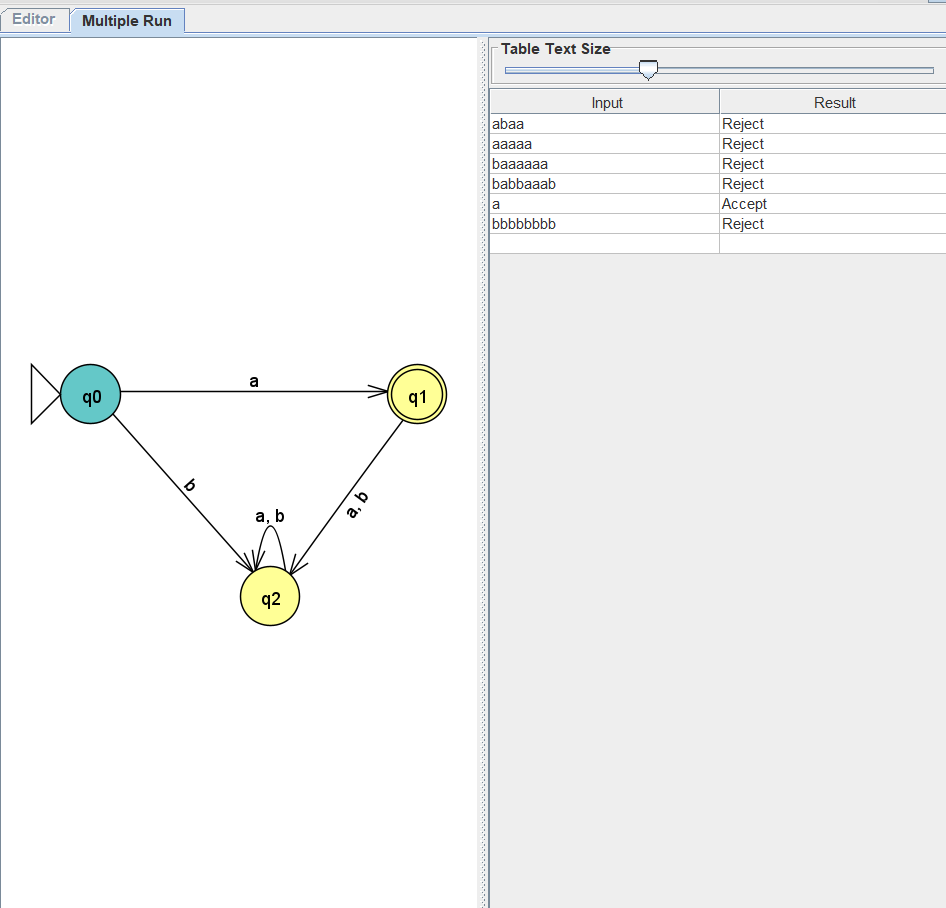
\includegraphics[width=0.5\textwidth]{AutomataEnJFLAP.png}
    \caption{Autómata en JFLAP}
    \label{fig:fig1}
\end{figure}

\textbf{Actividad 2:}
\begin{figure}[h]
    \centering
    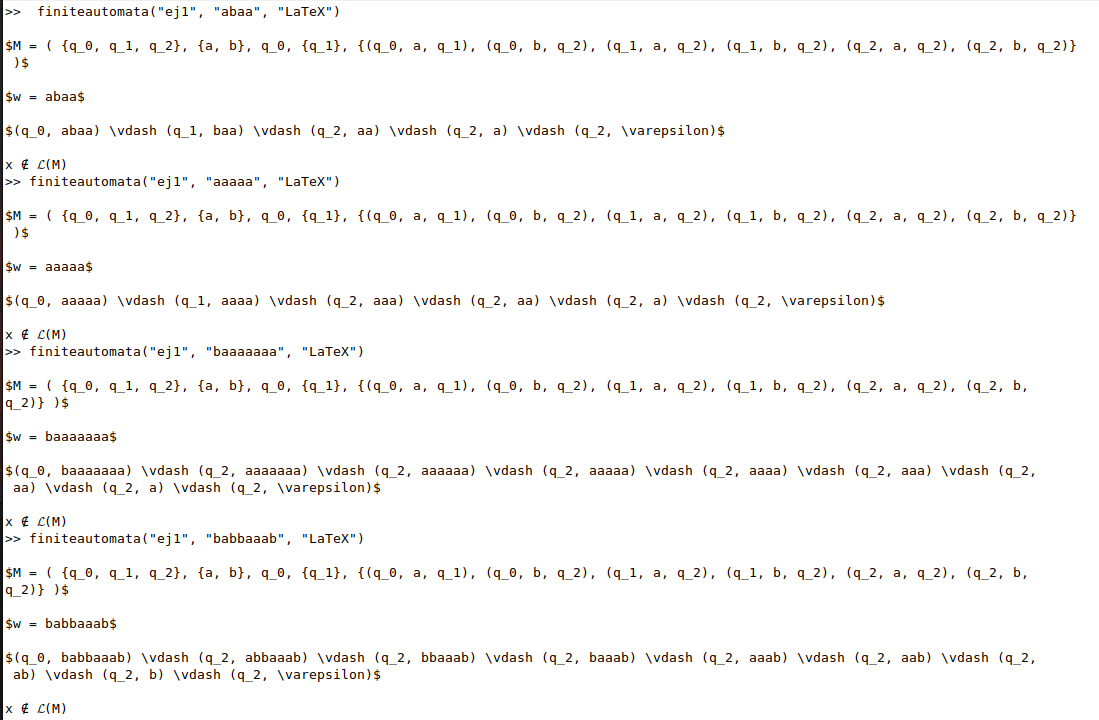
\includegraphics[width=0.8\textwidth]{AutomataenOctave1.png}
    \caption{Primeras 4 cadenas de prueba en Octave}
    \label{fig:fig2}
\end{figure}

\newpage

\textbf{Actividad 2:}
\begin{figure}[h]
    \centering
    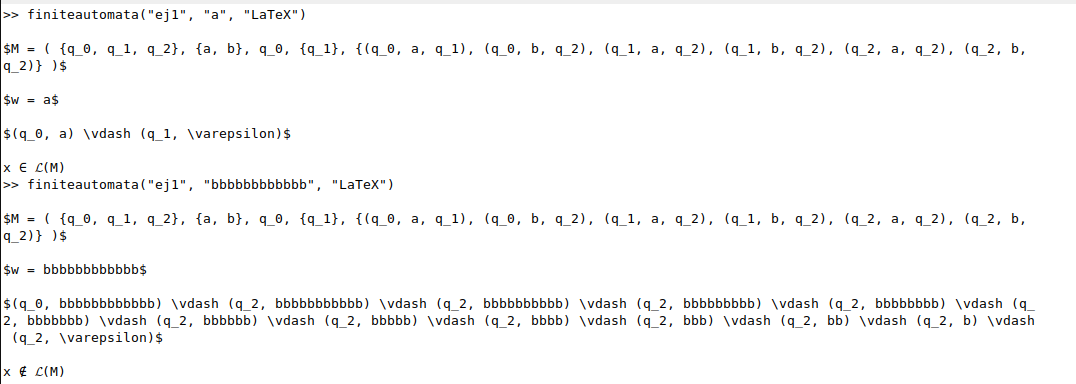
\includegraphics[width=0.9\textwidth]{AutomataenOctave2.png}
    \caption{Ultimas 2 cadenas de prueba en Octave}
    \label{fig:fig3}
\end{figure}

Como podemos observar, en la actividad 1 hemos creado un autómata finito determinista en el cual solo aceptara la cadena a sobre el lenguaje \{ a, b \} . En la imagen \ref{fig:fig1} podemos comprobar que la única cadena aceptada por el autómata es la cadena ' a .

En la segunda actividad, hemos comprobado que nuestro autómata estaba bien construido y hemos vuelto a ver si las cadenas probadas en el ejercicio 1 daban la misma solución.
En la imagen \ref{fig:fig2} ninguna de las cadenas es aceptada por el automata, mientras que en la imagen \ref{fig:fig3} vemos como la cadena ' a ' es aceptada por el lenguaje, por lo tanto hemos realizado con éxito estas actividades.



\end{document}
